\subsection{Detecting errors at runtime}
\begin{itemize}
	\item We want a means of recognizing and handling unusual conditions in your program at runtime, not just at compile time.
	\item A REQUIRES clause is just comments and cannot enforce the specification. Therefore, it is easy to pass parameters that violate the specification.
\end{itemize}

\subsection{Exceptions}
\begin{itemize}
	\item \textbf{Exceptions} let us detect an error in one part of the program and correct it in a different part of the program
	\item When an exception occurs, control transfers from normal-case code to the error handling code
	\item This error handling code then tries to correct the problem
	\begin{center}
		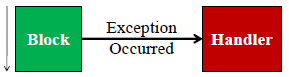
\includegraphics{sections/lec22/h.png}
	\end{center}
	\item When an exception occurs, it propagates from a function to its caller until it reaches a handler
	\item This is called \textbf{exception propagation}, and it happens automatically
\end{itemize}

\subsection{Exception Handling in C++}
\begin{itemize}
	\item When code detects an error, it uses a \lstinline[style=C++]{throw} statement
	\item Code that might cause an error goes in a \lstinline[style=C++]{try} block
	\item Code that corrects an error goes in a \lstinline[style=C++]{catch} block
	\item If the exception is successfully handled in the catch block, execution continues normally with the first statement following the catch block
	\item Otherwise, the exception is propagated to the enclosing block or to the caller if there is no enclosing block
	\item If an exception is propagated to the caller of \lstinline[style=C++]{main()}, the program exits
	\item When code detects an error, it uses a \lstinline[style=C++]{throw} statement
	\item When we throw an exception, we specify a value for the exception type in a throw statement
	\item e.g.,
\begin{lstlisting}[style=C++]
int n = 0; throw n;
char c = 'e'; throw c;
\end{lstlisting}
\end{itemize}

\subsection{Terminology}
\begin{itemize}
	\item Throw exception == raise exception
	\item Catch block == exception handler
\end{itemize}

\subsection{Exception Example}
\begin{itemize}
	\item Code that might cause an error goes in a \lstinline[style=C++]{try} block:
\begin{lstlisting}[style=C++]
int main() {
	string f; //function
	double n; //number
	
	while (cin>> f >> n) {
		try {
			if (f == "factorial") {
				cout<< factorial(n) << endl;
			}
		}catch(int i){
			cout << "try again" << endl;
		}
	}
}
\end{lstlisting}
	\item Code that corrects an error goes in a \lstinline[style=C++]{catch} block
	\item A \lstinline[style=C++]{catch} block goes directly after a \lstinline[style=C++]{try} block
	\item A \lstinline[style=C++]{catch} block matches the type from a \lstinline[style=C++]{throw} statement
\begin{lstlisting}[style=bash]
./a.out
factorial 5
120 
factorial -5
try again
\end{lstlisting}
	\item When an exception is not caught by a catch block, it propagates all the way to the caller of \lstinline[style=C++]{main}, and the program exits
\begin{lstlisting}[style=bash]
./a.out
combination -5 4
\item terminate called after thrown an instance of 'int'
Aborted (core dumped)
\end{lstlisting}
\end{itemize}

\subsection{Type discrimination}
\begin{itemize}
	\item A \lstinline[style=C++]{try} block can have multiple \lstinline[style=C++]{catch} blocks to handle different exception types
\begin{lstlisting}[style=C++]
try {
	if (foo) throw 4;
	// some statements go here
	if (bar) throw 2.0;
	// more statements go here
	if (baz) throw ‘a’;
}
catch (intn) { }
catch (double d) { }
catch (char c) { }
catch (...) { }
\end{lstlisting}
	\item The last handler is a \textbf{default handler}, which matches any exception type. It can be used as a ``catch-all'' in case no other catch block matches.
\end{itemize}

\subsection{Exception types}
\begin{itemize}
	\item Code often uses custom types to describe errors:
	\item e.g.,
\begin{lstlisting}[style=C++]
class NegativeError{};
class InputError{};
\end{lstlisting}
	\item We use the class mechanism to declare custom types
	\item When an error is detected, create a \lstinline[style=C++]{NegativeError} object and \lstinline[style=C++]{throw} it:
\begin{lstlisting}[style=C++]
//EFFECTS: returns n!, throws NegativeErrorfor n<0
int factorial (int n) {
	if (n<0) throw NegativeError();
	int result = 1;
	while (n > 0) {
		result *= n;
		n -= 1;
	}
	return result;
}

int main() {
	//...
	while (cin >> f >> n) {
		try {
			//...
		} catch (NegativeError){
			cout<< "try a positive number" << endl;
		} catch (...) {
			cout<< "try again" <<endl;
		}
	}
}
\end{lstlisting}
	\item See examples from lecture slides.
\end{itemize}